\noindent метить, \( S_1 + S_2 + . . . + S_n^1 = \Sigma_1 + . . . + \Sigma_n \), поэтому сумма, стоящая в левой части, также велика и, значит, одно из слагаемых, скажем \( S_l \), также велико. Аккуратное проведение доказательства мы предоставляем читателю. Перейдем теперь к решению задачи.

Р е ш е н и е \quad з а д а ч и. \quad Выпишем остатки от деления чисел \( 2^{l+1}, \dots , 2^{l+L} \) на \( m \) и будем ставить между двумя последовательными остатками «галочку», если первый больше второго. Тогда, во-первых, остаток, стоящий перед галочкой, больше \( \frac{m}{2} \), во-вторых, количество чисел между двумя последовательными галочками меньше \( \log_2 2m \), так как остатки между двумя галочками образуют геометрическую прогрессию со знаменателем \( 2 \) (действительно, \( 2\log_2 2m - 1=m > m-1 \), а всякий остаток не больше \( m-1 \)). Таким образом, число промежутков между галочками большее \( \frac{L}{\log_2 2m} - 1 \) и так как в конце каждого промежутка стоит число, больше \( \frac{m}{2} \), то все доказано.

\begin{flushright} \textsl{A. Г. Кушниренко} \end{flushright}

\vspace{0.5cm}

\textbf{В этом номере мы публикуем решения задач Ф43, Ф48—Ф51}

\begin{center} \textbf{Ф43} \end{center}

\begin{small} Найти давление в центре жидкой планеты радиуса \( R \), если жидкость несжимаема и имеет плотность \( p \). \end{small}

\vspace{0.2cm}

Разобьем объем планеты на тонкие сферические слои толщиной \( \Delta r \). Легко показать, что равнодействующая гравитационных сил, действующих со стороны слоя на частицу внутри этого слоя, равна нулю. Действительно, рассмотрим для этого конус с малым углом при вершине, в которую помещена частица массы \( m \). Конус вырезает из слоя участки площадями \( s_1 \) и \( s_2 \) (рис. 1). Если масса вещества, приходящегося на единицу поверхности слоя, равна \( \mu \), то гравитационные силы, действующие на массу \( m \) со стороны участков \( s_1 \) и \( s_2 \), равны

\begin{small} \[
F_1 = \gamma \frac{m \mu s_1}{r_1^2}, \quad F_2 = \gamma \frac{m \mu s_2}{r_2^2};
\] \end{small}

\vspace{0.2cm}

но

\[
\frac{s_1}{r_1^2} \cos \alpha_1 = \frac{s_2}{r_2^2} \cos \alpha_2 = \Omega
\]
(\(\Omega\) — телесный угол при вершине конуса), а \( \alpha_1 = \alpha_2 \); заштрихованные треугольники подобны, то есть \begin{small} \( \angle OA_1 M_1 = \angle OA_2 M_2, \quad \angle OA_1 B_1 = \angle OA_2 B_2 \) \end{small} (они опираются на одну и ту же дугу) и
\begin{small} \( \alpha_1 = \angle OA_1 B_1 - \angle OA_1 M_{\gamma} a \alpha_2 = \angle OA_2 B_2 - \angle OA_2 M_2. \) \end{small}
Поэтому \(\frac{s_1}{r_1^2} = \frac{s_2}{r_2^2}.\) Благодаря этому \( F_1 = F_2\), то есть эти силы взаимно уравновешивают друг друга. Проведя аналогичное рассмотрение для других участков слоя, мы и докажем сделанное утверждение.

Сила, с которой притягивается элемент слоя \( \Delta s \Delta r \) к центру планеты, равна

\[
F = \gamma \frac{\frac{4}{3} \pi r^3 \rho \Delta s \Delta r \rho}{r^2},
\]
где \( r \) — расстояние от этого элемента до центра планеты. Отсюда найдем, что увеличение давления на участке толщиной \( \Delta s \) равно

\[
\Delta p = \frac{F}{\Delta s} = \frac{4}{3} \pi \gamma \rho^2 r \Delta r.
\]
Поэтому давление на расстоянии \( r_0 \) от центра планеты будет равно

\[
p = p_0 + \frac{4}{3} \pi \gamma \rho^2 \Sigma r \Delta r.
\]

Так как сумма \( r \Delta r \) равна площади

\begin{figure}[h]
\centering
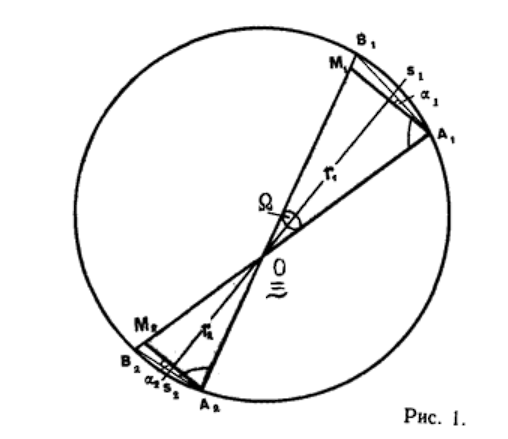
\includegraphics[width=1\linewidth]{рис1.png} 
\end{figure}

\begin{flushright} \begin{footnotesize} \textbf{35} \end{footnotesize} \end{flushright}

\newpage

\begin{table}
\centering
\renewcommand{\arraystretch}{1.5}

\begin{tabular}{|c|c|c|c|c|c|c|c|c|c|c|c|}
\hline
& 0 & 1 & 1 & 0 & 1 & 1 & 1 & 0 & 0 & 0 \\
\hline
0 & \cellcolor{white!30} $+$ & \cellcolor{blue!30} $-$ & \cellcolor{blue!30} $-$ & \cellcolor{white!30} $+$ & \cellcolor{blue!30} $-$ & \cellcolor{blue!30} $-$ & \cellcolor{blue!30} $-$ & \cellcolor{white!30} $+$ & \cellcolor{white!30} $+$ & \cellcolor{white!30} $+$ \\
\hline
0 & \cellcolor{white!30} $+$ & \cellcolor{blue!30} $-$ & \cellcolor{blue!30} $-$ & \cellcolor{white!30} $+$ & \cellcolor{blue!30} $-$ & \cellcolor{blue!30} $-$ & \cellcolor{blue!30} $-$ & \cellcolor{white!30} $+$ & \cellcolor{white!30} $+$ & \cellcolor{white!30} $+$ \\
\hline
1 & \cellcolor{yellow!30} $-$ & \cellcolor{green!30} $+$ & \cellcolor{green!30} $+$ & \cellcolor{yellow!30} $-$ & \cellcolor{green!30} $+$ & \cellcolor{green!30} $+$ & \cellcolor{green!30} $+$ & \cellcolor{yellow!30} $-$ & \cellcolor{yellow!30} $-$ & \cellcolor{yellow!30} $+$ \\
\hline
1 & \cellcolor{yellow!30} $-$ & \cellcolor{green!30} $+$ & \cellcolor{green!30} $+$ & \cellcolor{yellow!30} $-$ & \cellcolor{green!30} $+$ & \cellcolor{green!30} $+$ & \cellcolor{green!30} $+$ & \cellcolor{yellow!30} $-$ & \cellcolor{yellow!30} $-$ & \cellcolor{yellow!30} $-$ \\
\hline
0 & \cellcolor{white!30} $+$ & \cellcolor{blue!30} $-$ & \cellcolor{blue!30} $-$ & \cellcolor{white!30} $+$ & \cellcolor{blue!30} $-$ & \cellcolor{blue!30} $-$ & \cellcolor{blue!30} $-$ & \cellcolor{white!30} $+$ & \cellcolor{white!30} $+$ & \cellcolor{white!30} $+$ \\
\hline
1 & \cellcolor{yellow!30} $-$ & \cellcolor{green!30} $+$ & \cellcolor{green!30} $+$ & \cellcolor{yellow!30} $-$ & \cellcolor{green!30} $+$ & \cellcolor{green!30} $+$ & \cellcolor{green!30} $+$ & \cellcolor{yellow!30} $-$ & \cellcolor{yellow!30} $-$ & \cellcolor{yellow!30} $-$ \\
\hline
0 & \cellcolor{white!30} $+$ & \cellcolor{blue!30} $-$ & \cellcolor{blue!30} $-$ & \cellcolor{white!30} $+$ & \cellcolor{blue!30} $-$ & \cellcolor{blue!30} $-$ & \cellcolor{blue!30} $-$ & \cellcolor{white!30} $+$ & \cellcolor{white!30} $+$ & \cellcolor{white!30} $+$ \\
\hline
1 & \cellcolor{yellow!30} $-$ & \cellcolor{green!30} $+$ & \cellcolor{green!30} $+$ & \cellcolor{yellow!30} $-$ & \cellcolor{green!30} $+$ & \cellcolor{green!30} $+$ & \cellcolor{green!30} $+$ & \cellcolor{yellow!30} $-$ & \cellcolor{yellow!30} $-$ & \cellcolor{yellow!30} $-$ \\
\hline
0 & \cellcolor{white!30} $+$ & \cellcolor{blue!30} $-$ & \cellcolor{blue!30} $-$ & \cellcolor{white!30} $+$ & \cellcolor{blue!30} $-$ & \cellcolor{blue!30} $-$ & \cellcolor{blue!30} $-$ & \cellcolor{white!30} $+$ & \cellcolor{white!30} $+$ & \cellcolor{white!30} $+$ \\
\hline
0 & \cellcolor{white!30} $+$ & \cellcolor{blue!30} $-$ & \cellcolor{blue!30} $-$ & \cellcolor{white!30} $+$ & \cellcolor{blue!30} $-$ & \cellcolor{blue!30} $-$ & \cellcolor{blue!30} $-$ & \cellcolor{white!30} $+$ & \cellcolor{white!30} $+$ & \cellcolor{white!30} $+$ \\
\hline
\end{tabular}
\end{table}

\begin{figure}
\caption{рисунок}
\end{figure}

\noindent щее количество минусов в полученной таблице зависит только от четности чисел \( x_i \) и \( y_k \); на рисунке 1 вместо четных чисел поставлены нули, вместо нечетных --- единицы. Пусть \( x \) --- число нечетных чисел среди \( x_i \); \( y \) --- число нечетных чисел среди \( y_k \) (на рисунке \( x = 5, \, y = 4 \)). Тогда, как нетрудно посчитать, общее число минусов в таблице будет равно

\[
x(100 - y) + (100 - x)y = 100x + 100y - 2xy,
\]
где \( x, \, y \) --- целые.

Теперь вернемся к нашей задаче и докажем, что ответ в ней отрицательный, т.~е. 1970 минусов получить невозможно. Предположим, что нам удалось получить ровно 1970 минусов. Тогда \( 1970 = 100x + 100y - 2xy \), откуда

\[
xy - 50x - 50y + 2500 = 1515.
\]

Разложив левую часть на множители, получаем
\[
(x - 50)(y - 50) = 1515 = 15 \cdot 101.
\]

Имеем
\[
-50 \leq x - 50 \leq 50, \quad -50 \leq y - 50 \leq 50.
\]

$$\int_1^1$$ $$\int\limits_1^2$$